\documentclass{article}
\usepackage{graphicx} % Required for inserting images
\usepackage{graphicx}
\usepackage{fancyhdr}

\pagestyle{fancy}
\fancyhf{}
\fancyhead[L]{DEIN UT4}
\fancyhead[R]{Adrian García DAM 2B}
\rfoot{\thepage}


\title{Filmosis}
\author{Proyecto Intermodular DAM, Maria Ana Sanz}
\date{Curso 2023-2024}

\begin{document}

\begin{titlepage}
    \centering

    \maketitle

    
\includegraphics[width=0.8\textwidth]{images/logo_ci_mas.jpg}

    \vspace{1cm}
    
    
\includegraphics[width=0.8\textwidth]{images/logoFilmosisPremium.png}
    
    \vspace{1cm}
    
    \textbf{Integrantes}
    
    \vspace{0.5cm}
    
    \begin{minipage}{0.5\textwidth}
        \centering
        Jiménez Aldasoro, Kaiet \\
        Arrondo Villaplana, Aritz \\
        García Galera, Adrián
    \end{minipage}
    
\end{titlepage}

\renewcommand{\contentsname}{Índice}
\tableofcontents

\newpage

\section{Descripción}

Filmosis es una aplicación dedicada a los amantes del cine que buscan una experiencia completa para descubrir, explorar y valorar películas. Esta plataforma combina la riqueza de información de IMDb con una función de valoración integrada, permitiendo a los usuarios sumergirse en el vasto mundo del cine de una manera interactiva y social.

Características destacadas:

\begin{itemize}
    \item Exploración de Películas: Filmosis ofrece una amplia base de datos de películas donde los usuarios pueden explorar información detallada sobre películas, desde el elenco hasta las críticas.
    
    \item Sistema de Valoración: Los usuarios pueden calificar y revisar películas, compartiendo sus opiniones con la comunidad de Filmosis. La función de valoración permite a los usuarios descubrir películas populares y apreciadas por otros miembros de la plataforma.
    
    \item Listas Personalizadas: Los usuarios pueden crear listas personalizadas de películas, como "Mis Favoritas", "Por Ver", o cualquier categoría que deseen. Esta función ayuda a organizar y compartir preferencias cinematográficas.
    
    \item Noticias y Actualizaciones: Filmosis mantiene a los usuarios actualizados sobre las últimas noticias y eventos en la industria cinematográfica, asegurándose de que estén informados sobre estrenos, premios y más.
    
    \item Perfil de Usuario: Cada usuario tiene su propio perfil personalizado, donde pueden ver sus valoraciones, listas y contribuciones. También pueden conectarse con amigos y descubrir lo que están viendo y valorando.
\end{itemize}

Filmosis se esfuerza por crear una comunidad vibrante de cinéfilos, proporcionando una plataforma interactiva y social para explorar y disfrutar del mundo del cine.

\vspace{1cm}

\begin{minipage}{1\textwidth}
    \centering
    
\includegraphics[width=0.6\textwidth]{images/logoFilmosis.png}
\end{minipage}

\section{Arquitectura}

La arquitectura de Filmosis está diseñada para ofrecer una experiencia completa a los usuarios amantes del cine, utilizando diversas tecnologías y servicios. A continuación, se presenta una descripción de la arquitectura:

\begin{itemize}
    \item Main Activity y Fragmentos: La aplicación Filmosis utiliza un diseño de interfaz basado en una MainActivity que contiene varios fragmentos. Estos fragmentos representan las distintas secciones de la aplicación, como la pantalla de inicio, la pantalla de búsqueda, la pantalla de listas personalizadas y la pantalla de perfil de usuario. Este enfoque modular facilita la gestión y la navegación en la aplicación.
    
    \item Retrofit para Peticiones a APIs: Filmosis utiliza la biblioteca Retrofit para realizar peticiones a la API de The Movie Database (TMDb). Retrofit simplifica la interacción con servicios web al convertir las solicitudes HTTP en llamadas a métodos de Java, facilitando la integración y la gestión de datos externos.
    
    \item The Movie Database (TMDb): Filmosis se integra con The Movie Database (TMDb) para obtener información detallada sobre películas, desde detalles de la trama hasta elenco, críticas y más. TMDb proporciona una amplia base de datos cinematográfica que enriquece la experiencia de los usuarios al ofrecer información precisa y actualizada.
    
    \item Firebase para la Base de Datos y Usuarios: Filmosis utiliza Firebase como plataforma integral para gestionar la base de datos y la autenticación de usuarios. Firebase Realtime Database almacena datos en tiempo real y permite sincronizar la información entre diferentes dispositivos de forma eficiente. Además, Firebase Authentication proporciona un sistema seguro para la gestión de usuarios, permitiendo a los usuarios crear perfiles personalizados, calificar películas y gestionar sus listas personalizadas.

\end{itemize}

\vspace{1cm}

\begin{minipage}{1\textwidth}
    \centering
    
\includegraphics[width=0.4\textwidth]{images/arquitecturaSoftware.png}
\end{minipage}

\section{Diseño}

\subsection{Pantalla Inicial}

    \begin{minipage}{0.4\textwidth}
        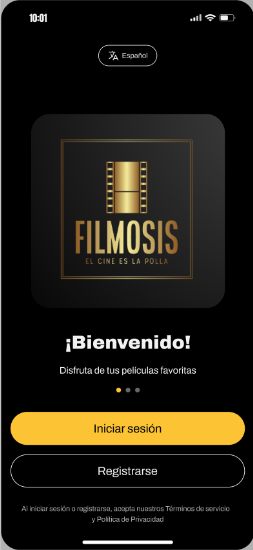
\includegraphics[width=\textwidth]{images/pantallaInicio.png}
    \end{minipage}
    \hfill
    \begin{minipage}{0.55\textwidth}
    La pantalla de inicio contendrá el logo de la aplicación, junto con un mensaje de bienvenida.
    
    Además, tendrás la opción de iniciar sesión o de registrarse, aceptando los términos de servicio y política de privacidad.
    
    También dispone de un botón en la parte superior para cambiar el idioma.
    
    \end{minipage}

\subsection{Pantalla de Registro}

    \begin{minipage}{0.4\textwidth}
        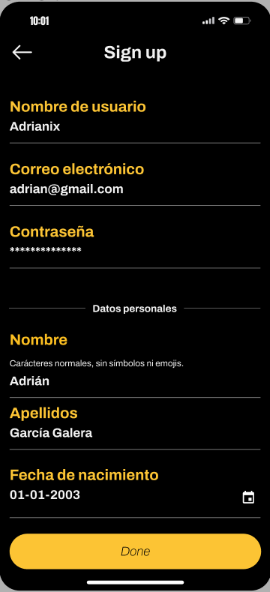
\includegraphics[width=\textwidth]{images/pantallaRegistro.png}
    \end{minipage}
    \hfill
    \begin{minipage}{0.55\textwidth}
    La pantalla de registro contiene 6 campos con diferentes requisitos.
    
    La primera parte consiste en los datos acerca de la cuenta, como son el nombre de usuario, correo electrónico y contraseña.
    
    Después, hay que rellenar datos personales, los cuáles son el nombre, apellidos y fecha de nacimiento.

    
    \end{minipage}

\subsection{Pantallas de Listas Personalizadas}

    \begin{minipage}{0.4\textwidth}
        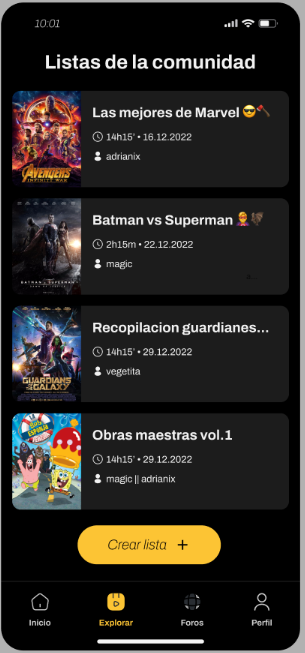
\includegraphics[width=\textwidth]{images/pantallaListas.png}
    \end{minipage}
    \begin{minipage}{0.55\textwidth}
    Esta pantalla contendrá listas creadas por los usuarios, las cuales se podrán consultar y guardar si se desea.
    
    \end{minipage}
    \hfill

\subsection{Pantalla de Home}

    \begin{minipage}{0.4\textwidth}
        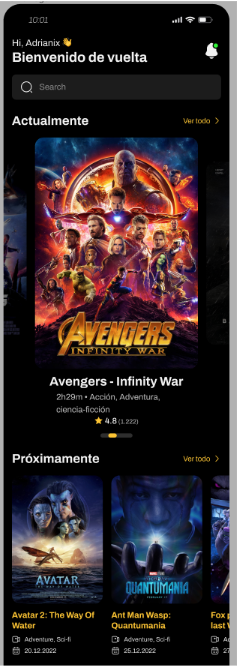
\includegraphics[width=\textwidth]{images/pantallaHome.png}
    \end{minipage}
    \hfill
    \begin{minipage}{0.55\textwidth}
    La pantalla de inicio consiste en cinco secciones:
        \begin{itemize}
            \item Actualmente: En donde se listarán las películas en cartelera actuales
            \item Próximamente: Las futuras películas 
            \item Populares: Las películas más populares del momento
            \item Servicios: Para buscar el contenido mas popular por cada plataforma
            \item Noticias: Últimas noticias de películas.
        \end{itemize}
    
    \end{minipage}

\subsection{Pantalla de Foros}

    \begin{minipage}{0.4\textwidth}
        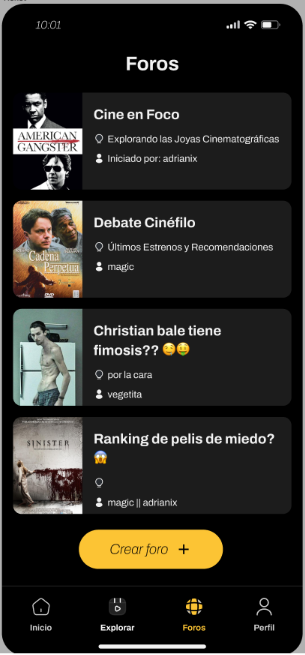
\includegraphics[width=\textwidth]{images/pantallaForos.png}
    \end{minipage}
    \hfill
    \begin{minipage}{0.55\textwidth}
    La pantalla de foros contendrá foros para conversar con diferentes usuarios y discutir acerca de distintos temas.
    
    La estructura es parecida a la pantalla de listas personalizadas.

    \end{minipage}

\subsection{Pantalla de Película Seleccionada}

    \begin{minipage}{0.4\textwidth}
        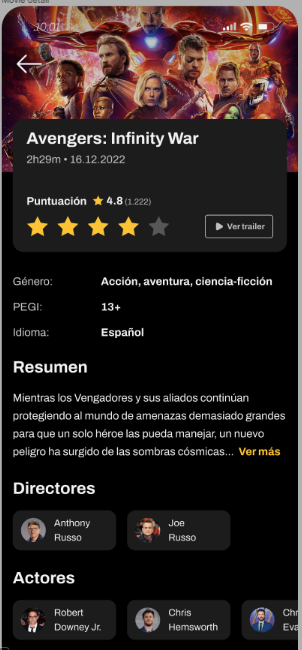
\includegraphics[width=\textwidth]{images/pantallaPeliSeleccionada.png}
    \end{minipage}
    \hfill
    \begin{minipage}{0.55\textwidth}
    Las pantalla de película seleccionada contiene información variada acerca de la película, como su puntuación y el resumen, los directores y actores, o los servicios en donde está disponible
    
    \end{minipage}

\newpage

\section{Conclusión}

En resumen, Filmosis se presenta como una aplicación integral diseñada para los amantes del cine, ofreciendo una experiencia completa que combina la riqueza informativa de IMDb con características sociales interactivas. Los usuarios pueden explorar una extensa base de datos de películas, accediendo a detalles como el elenco y las críticas. La función de valoración permite a los usuarios compartir sus opiniones, descubrir películas populares y conectarse con la comunidad. La posibilidad de crear listas personalizadas facilita la organización y compartición de preferencias cinematográficas. Además, Filmosis mantiene a los usuarios informados sobre las últimas noticias y eventos en la industria cinematográfica. Con perfiles de usuario personalizados, la aplicación busca fomentar una comunidad vibrante de cinéfilos, ofreciendo una plataforma interactiva y social para explorar y disfrutar del mundo del cine.

\end{document}
